\documentclass{beamer}
\usepackage[english,russian]{babel}
\usepackage[utf8]{inputenc}
\usepackage{amsmath}
\usepackage{hyperref}
\usetheme{Warsaw}
\usepackage{listings}
\usepackage{xcolor}
\usepackage{tikz}
\usetikzlibrary{graphs}
\usepackage{algpseudocode}

\lstset{
    frame=tb,
    tabsize=4,
    showstringspaces=false,
    numbers=left,
    commentstyle=\color{green},
    keywordstyle=\color{blue},
    stringstyle=\color{red},
    emph={baz},
    emphstyle=\textbf
}

\begin{document}

\title{SAT/SMT solvers\newline  8. Quantified Formulas}
\author{Roman Kholin}
\institute{Lalambda}
\date{Tbilisi, 2023}

\begin{frame}
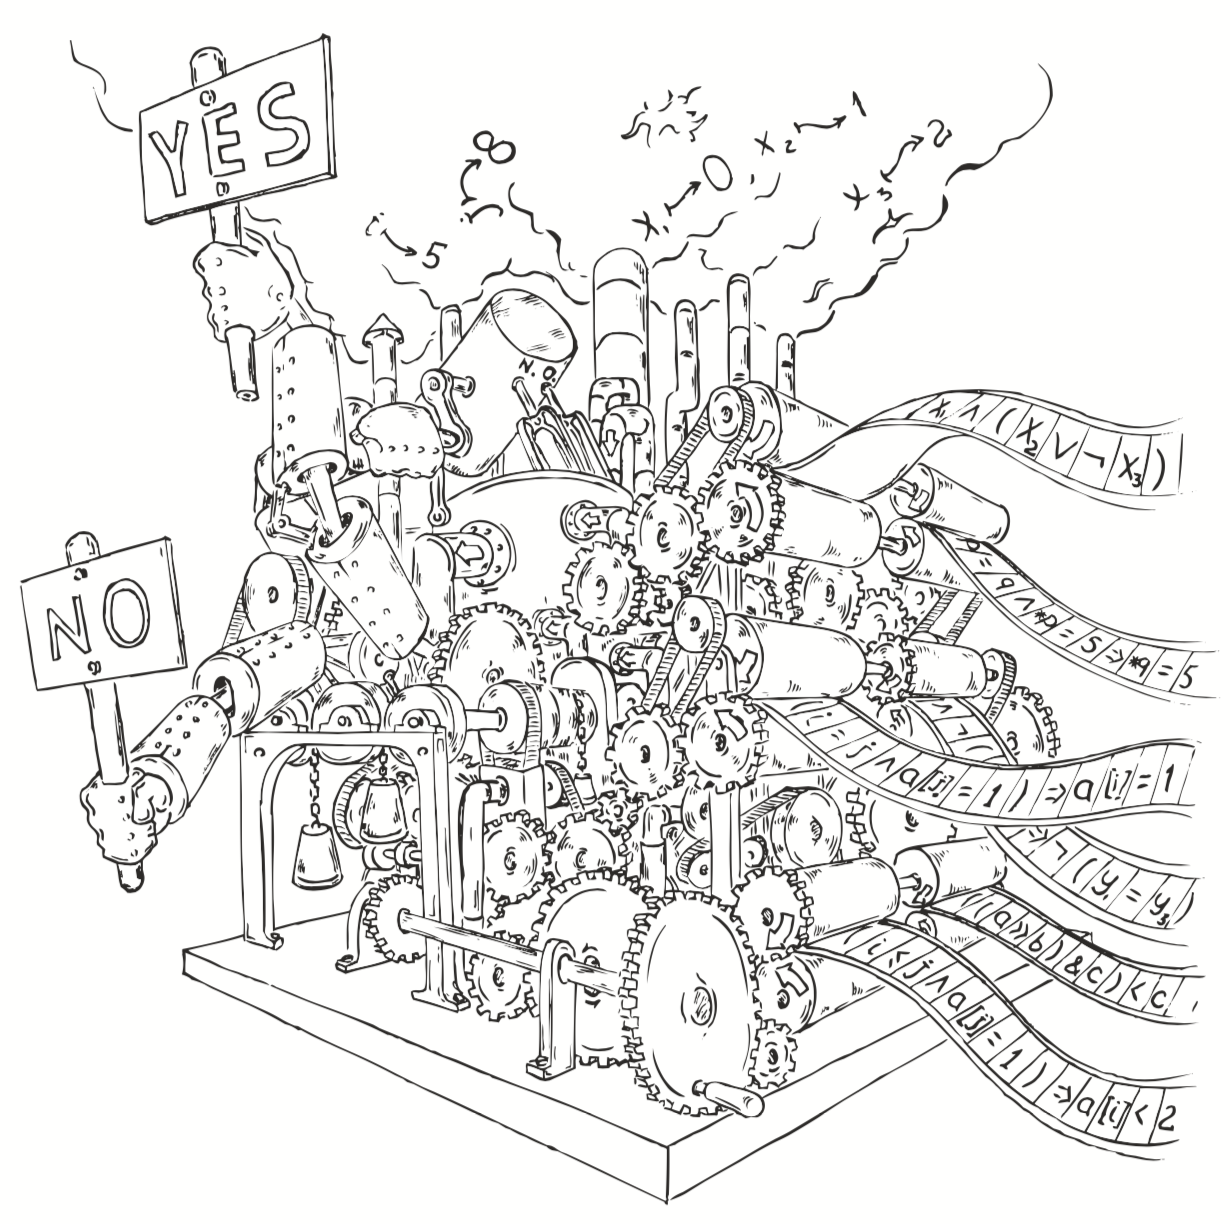
\includegraphics[scale=0.5]{../decision-procedure.png}
\end{frame}

\frame{\titlepage}

\begin{frame}{Definitions}
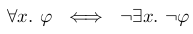
\includegraphics[scale=0.5]{all_and_exist.png}\newline
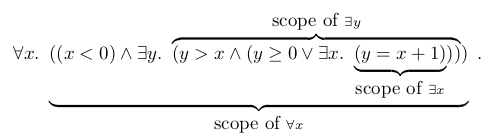
\includegraphics[scale=0.5]{scope.png}\newline
\begin{block}{}
\begin{itemize}
\item A variable is called free in a given formula if at least one of its occurrences is not bound by any quantifier
\item A formula Q is called a sentence (or closed) if none of its variables are free
\end{itemize}
\end{block}
\end{frame}

\begin{frame}{Syntax}
QBF:\newline
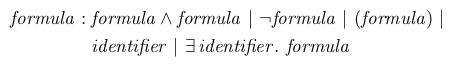
\includegraphics[scale=0.5]{qbf.png}\newline
Complexity - PSPACE\newline
QDLA:\newline
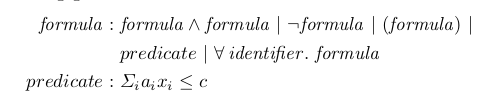
\includegraphics[scale=0.5]{qdla.png}\newline
\end{frame}

\begin{frame}{Definitions}
\begin{block}{Prenex normal form}
\begin{itemize}
\item A formula is said to be in prenex normal form (PNF) if it is in the form $Q[n]V[n]\dots Q[1]V[1].<quantifier-free formula>$, where $Q[i]$ - quantor, $V[i]$ - variable
\item For every quantified formula Q there exists a formula Q' in prenex normal form such that Q is valid if and only if Q' is valid
\end{itemize}
\end{block}
\end{frame}

\begin{frame}
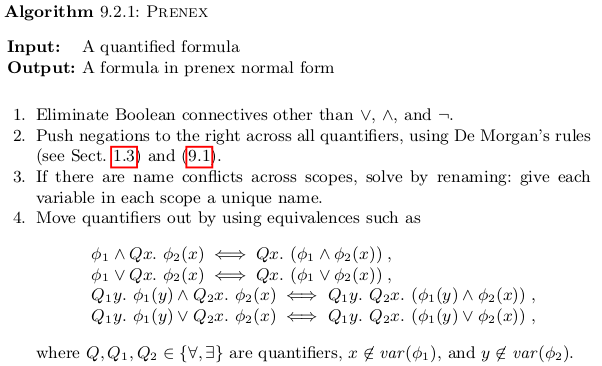
\includegraphics[scale=0.5]{prenex.png}\newline
\end{frame}

\begin{frame}{Example}
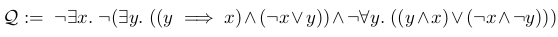
\includegraphics[scale=0.5]{prenex_example.png}\newline
\end{frame}

\begin{frame}{Projection}
Projection of $Q[n]V[n]\dots Q[2]V[2].\exists x.\phi$\newline
is $Q[n]V[n]\dots Q[2]V[2].\phi$
\end{frame}

\begin{frame}{Example}
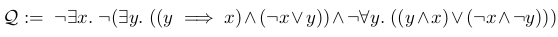
\includegraphics[scale=0.5]{prenex_example.png}\newline
\end{frame}

\begin{frame}
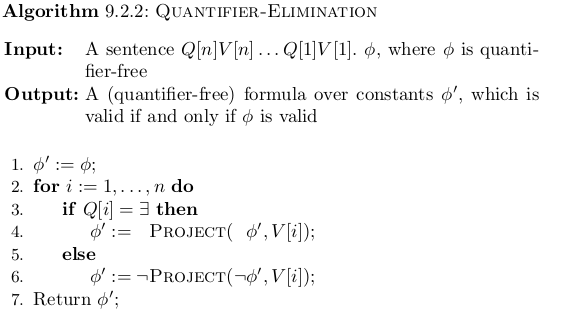
\includegraphics[scale=0.5]{quantifier-elimination.png}\newline
\end{frame}

\begin{frame}{Quantifier elimination for Quantified Boolean Formulas}
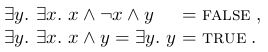
\includegraphics[scale=0.5]{elem_qbf1.png}\newline
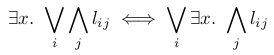
\includegraphics[scale=0.5]{elem_qbf2.png}\newline
\end{frame}

\begin{frame}
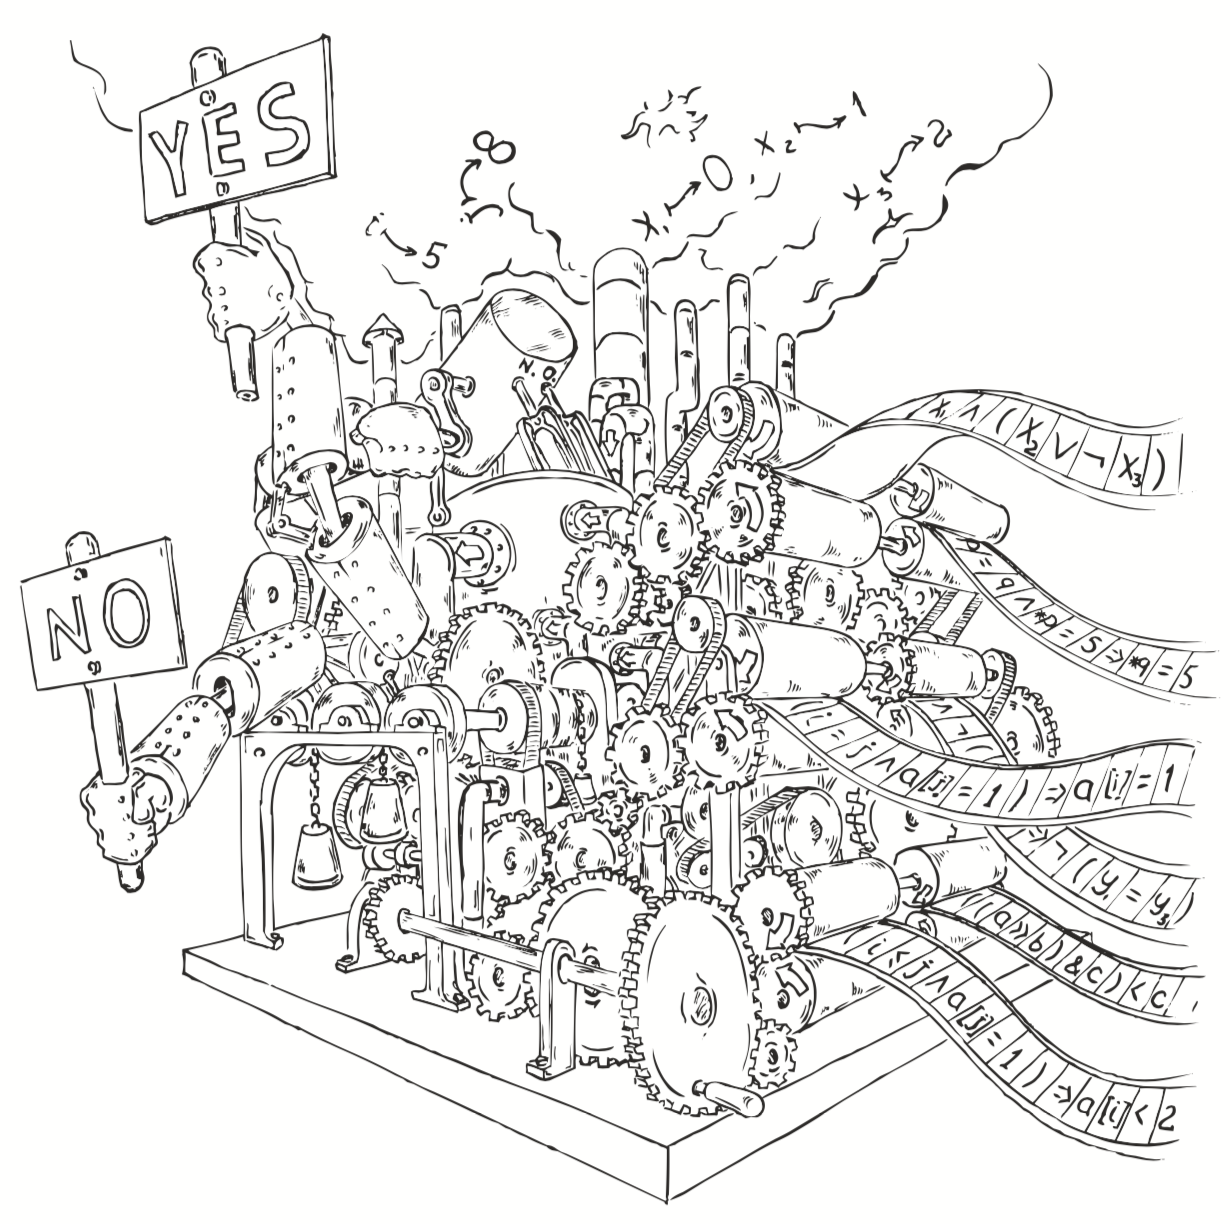
\includegraphics[scale=0.5]{../decision-procedure.png}
\end{frame}

\end{document}
